
%\chapter{The effect of phenotypic plasticity on plant community dynamics}
%Hypothesis on the cumulative effect on niche and interactions.
%
%\section{Individual resistance and resilience against drought events}
%Amplitude and length of the event :\\
%- severity effect reduced by lower tau ?\\
%- resistance versus resilience: H0: conservative strategy have higher resistance, H1 : low tau allows for re-equilibrium and increase resistance (low amplitude and long length. H2: high tau allow to avoid dead-end situation during short severe drought (high resilience)
%\section{Community response to drought event}
%coexistence effect vs resistance/resilience effect\\
%uniform vs heterogenous (plasticity wise) community response
%H1: 
%

\begin{fullwidth}
This second result chapter examines the effects of the phenotypic plasticity at the scale of the community. Another parameter filtering processes is performed and described in the first section of this chapter. The second part focuses on the effects of the plasticity on the main properties of the community. The impact of the plasticity on species diversity is particularly investigated. This chapter gives a glimpse of the potential of the model to answer various questions around the role of intraspecific variations on diverse community properties.
\end{fullwidth}

\chapter{Community level simulations: non plastic community}


\section{Parameter filtering}
\subsection{Method}

%\paragraph{Field data}
%Field data has been collected between years 201 .. and 201 by Claire Deleglise and al. (). Not used here.

\paragraph{Weather data}
Weather data for the time period between 1959 and 2014 has be computed by the MeteoFrance model SAFRAN by Déborah Verfaille using GPS coordinates, slope, azimuth and horizon computed from a digital elevation model. These parameters were also used by the model CROCUS to compute the snow accumulation and the snow melting. These high frequency data (resolution under 1h) have been averaged on a daily time-step and used to compute input variables for \model. The snow in particular defines the length of the growing season starting with the first snow melt of the year and finishing the day of the first snow fall during the autumn or winter. The simulated years above 2014 are randomly sampled form the existing dataset between 1995 and 2014.

The six sites have been chosen to test the consistency of the parameters, and open the door to the exploration of the effect of the climatic variables. This last aspect is not developed in this manuscript.

\paragraph{Parameter filtering}
A community level parameter filtering is conduced for a new table of parameter sets. The tested parameter sets are composed of all the parameter sets accepted at the individual-scale with 50 randomly sampled among the rejected parameter sets. They are completed with five community-level parameters: seed germination density, drought mortality, ageing mortality, plasticity cost for environmental sensing and plasticity cost for trait changes (see chapter \ref{chapter:model-description} for details). The values of these community-level parameters are randomly sampled with a LHS procedure.

\paragraph{Simulations}
The simulations run over 300 hundreds years for 6 sites with similar soil depth, but contrasted climate, on squares of 2,500 square centimetres, under \textit{non plastic} allocation algorithm. After a stabilising phase of 50 years, the simulation is stopped and the parameter set rejected if no individual persist and the seedbank is empty. The seedrain is composed of seeds contained in the seedbank and seeds from the metacommunity. The total of seeds is defined by the seed germination density and the area simulated. The seeds from the simulated community represent up to 80 \% of the seedrain, less if the seed production is limiting. 400 species compose the meta-community with traits randomly sample from distributions estimated from the accepted parameter sets at the individual scale. More complex procedure could be imagine to better take benefit of the information extracted from the individual-level calibration. This method is preferred because only one species is evaluated for each parameter set at the individual-level, thus no distribution specific to each parameter set could be used. This method still allows to avoid traits values that make no sense in any of the parameter set and reduces, even marginally, the number of potential non-viable species.



\subsection{Results}


\paragraph{Parameter filtering}

Among the  tested parameter sets, only 77 were selected after the parameter filtering process. 

Because too few parameter sets are selected with contrasted parameter values, no sensitivity analysis could be conduced to determined the key parameters of the model. For the same reason, the parameter effects are not detailed.

\paragraph{General behaviour}

While the main properties of the simulated communities are explored in the following subsection, the general community growth can be observed for these simulations. The individual profiles show a relatively high variability within the season, that is coupled with high inter-site and/or inter-seasonal variability for any given parameter set.
Despite variable growing-season starting dates, and some variability within parameter sets, the smoothed-profile show a consistent behaviour. This pattern is characterised by two distinct growth periods: (1) the initial growth  corresponding to the use of the stored resources, then followed by the growth promoted by the favourable conditions of the spring and early summer, and (2) another growth period at the end of the summer/autumn, following the growth reduction of the mid-summer. Two peaks can be observed during the first phase, but the first one is only noticeable for a few conditions where the season started early.  

\begin{figure}%[tb]
%    \classiccaptionstyle
%\sidebysidecaption{0.5\textwidth}{0.4\textwidth}{%
    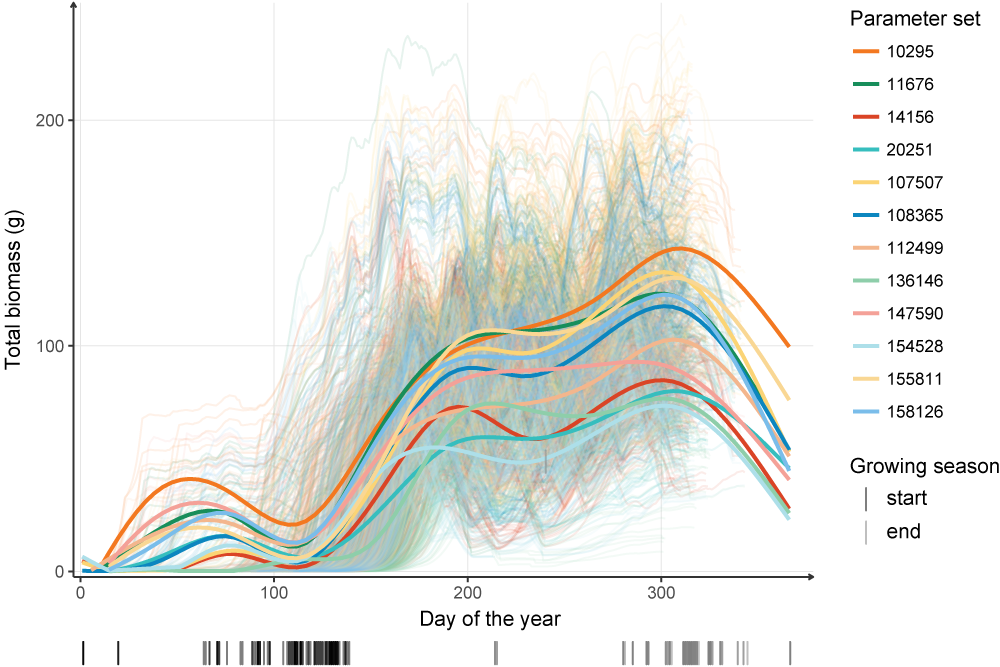
\includegraphics[width=1\linewidth]{./2_PP/Figures/Comm/biomass_season_non_plastic2.png}%
%}{%
  \caption[Total biomass over time during the growing season for the \textit{non palstic}allocation.]{Total biomass over time during the growing season for the \textit{non palstic}allocation. The thin lines illustrate the individual seasons profiles (n = 20) for different sites (n=6) and parameter sets (colour). The growth profile of the different parameter sets are estimated with GAM models. The marks at the bottom indicate the beginning and the end of the seasons.}
  \label{fg:species_per_plant}
%  }
\end{figure}

\subsection{Discussion}

\paragraph{Parameter filtering}

The parameter filtering process deployed here is sufiscient to select viable parameter sets allowing stable simulations. Ones could develop extended calibration plans to stabilise the behaviour of the model and ensure more realistic output. However, such approaches are mostly interesting when the model is built to infer information about specific, well described systems, instead of qualifying the general effect of freshly modelled mechanisms. The non reduction of the analysis of the model to one parameter set also increase the confidence in the observed pattern, and the conviction that they emerge from its structure rather than specific parameter interactions. Moreover, ambitious calibration procedure should rather be reserved to mature models, from which the general responses are well described and understood.

\paragraph{Driven by the weather}

The biomass profiles of the simulated communities show both consistency in the growth pattern, and high daily variability. The variability observed highlights the great the sensitivity to the weather variables. This sensitivity certainly favours positive effects of the phenotypic plasticity, if the changes in phenotype are responsive enough and do not suffer from a lag.

The consistent growth patter with two distinct growth period correspond to field observations where plants are generally divided between early flowering, matching the first biomass peak, and late flowering corresponding to an autumn growth and reproduction. This coherent behaviour, driven by the climate gives confidence in the integration of the climatic variables as drivers of the community. Further work could be done to confirm the respective role of the temperature and precipitation, but this work focuses on the effect of phenotypic plasticity and both the relative sensitivity to the daily variations in the conditions and the importance of the climatic variables as driving forces supposes that the plasticity has the potential to affect the mountain communities.
% sensitivity to the weather
% general climate driven response.

\textbf{The parameter filtering at the community scale ensure stability of the simulations at the community level. It also gives confidence in the global behaviour of the model, and in the driving role of the climatic variables.}
%\section{Non plastic communities}
%Trade-off, diversity, stability ...
%
%
%\paragraph{Ecological trade-off ?}
%Is there a selection of some parameters ? Are there ecological trade-off (resource use strategy and reproduction) emerging from the model ?

\chapter{Plasticity: impact on species fitness and diversity}

After a simple parameter filtering, guaranteeing the stability of the communities, the effect of the plastic allocation algorithms can be investigated as the community level. In a same way as the previous section, the focus is given to the main properties of the community: the diversity, the productivity and the identity. 
%
%Plasticity in integrated framework and full community simulations. Plasticity mechanisms, but also plasticity as a strategy (look at the cost and tau). 
%
%Effects on productivity and coexistence. Difference in the correlation ?
%
%Effect of tau on persistence.

\section{Plasticity and diversity}


\subsection{Method}

\paragraph{Simulations}
To test the effect of plasticity on coexistence and community dynamics, runs from the parameter filtering are used as starting points to limit the simulation time of the stabilisation phase. For each parameter set tested, 6 different sites were tested during the calibration phases, 77 parameter sets were accepted and a sample of 18 parameter sets were tested, resulting in 108 communities. Each of those is the starting point of three parallel runs that differ only by the allocation algorithm used: \textit{non plastic}, \textit{fixed-equilibrium} and \textit{plastic-optimisation}. The \textit{fixed-equilibrium} is favoured to \textit{fixed-optimisation} algorithm because previous part of the document focused on this algorithm and because it is simpler to analyse. The \textit{plastic-optimisation} algorithm is simulated despite the relatively poor performance results observed in constant conditions and the high convergence. This is justified by the introduction of plasticity cost, continuous species specific plasticity ($0 < \tau < 1$) and temporal and spatial heterogeneity that should mitigate the negative sides of this allocation mechanism and give information of processes at stake.

The plasticity costs (maintenance: related to the value of $\tau$, and displacement: relative to changes in phenotypes) defined in the parameter sets are applied to all algorithms. In the \textit{non plastic} simulations, this results in an artificial additional cost to all species, especially those with a low value for $\tau$, but with no potential gain from plasticity as the allocation is non plastic. This choice was made to ensure that the differences between the simulations are the results of the allocation algorithm only, and not a cumulative effect of the algorithm and the plasticity costs that could not be disentangled. This artificial cost can be seen as an artificial abiotic filtering process. Because 400 species are present in the meta-community, enough species with high values of tau should be able to invade the habitats, limiting behaviour emerging from low sampling.


%\paragraph{Statistical tests}

%The differences of effects between the different types of plasticity on the variables of interest are computed unpaired Wilcoxon tests assuming an independence of the the different data points. This assumption of statistical independence is justified by the normalisation for each parameter set of the variables relative to the mean of the \textit{non plastic} group. This normalisation allows to compare the simulations between the parameters sets. The interactions and other level (site, and autocorrelations) are discussed later in this section.

\paragraph{Normalisation}
To allow comparison between the datasets, the variables are normalised over the mean value of the variable under \textit{non plastic} allocation. So the \textit{non plastic} algorithm is the reference, but the variability caused by sites and seasons is still visible.

The normalisation $Vn_{a, p, t, s}$ of the variable $V$ for the allocation algorithm $a$, the parameter set $p$, the time $t$ and the site $s$ is given by the following formula:

\begin{align}
Vn_{a, p, t, s} &= \frac{V_{a, p, t, s}}{ \bar{V} }\\
\bar{V} &= \frac{\sum_{a == \text{\textit{non plastic}}}{} Vn_{p, t, s} }{n}
\end{align}

where $n$ is the number of observations for the \textit{non plastic} algorithm.

\paragraph{Species \& trait values}

For practical reasons the entire composition during the season are not store during the simulation process. The trait values are estimated \textit{a posteriori} from the reproduction pool composed of living individuals and seed produced. The species default values are use to compute the community weighted mean of traits with the living biomass or the cumulative seed biomass. Therefore, even if under \textit{plastic-optimisation} allocation the plants can change their trait values, these changes are not measured.

\paragraph{Diversity measures}

The diversity indexes are computed from the reproduction pool (defined above). The \textit{alpha} diversity is simple expressed as the mean number of species per site and per year. The \textit{beta} diversity is defined as the total number of species divided by the \textit{alpha} diversity minus one. 

The abundance ranking is computed from the reproduction output, under the hypothesis that the reproductive output is proportional to the realised abundance and constitute a good proxy for the fitness.

\subsection{Results}

%Need to run the simulations. Script is almost ready, parameters are filtered from previous step.
%
%\paragraph{General behaviour} ?
%gradient along climatic gradient ? did I save the climate ? Nope, can't really say anything about it.

\paragraph{Effect on coexistence}

The level of coexistence is evaluated by the number of distinct species that manage to maintain at least one individual or produce at least one seed at the end of the season. This criterion allows to ignore the potential non stable diversity introduced by the meta-community invasion (sampling of species in the meta-community pool) and to consider species that can be filtered out due to seed mortality. The number of species increases in almost all simulated years and sites for both plastic allocation algorithms, with a median of 1.5 times the number of species in \textit{non plastic} simulations (see figure \ref{fig:species_richness}). This factor can go up to 6 for \textit{fixed-equilibrium} and 9 for \textit{plastic optimisation}.


\begin{marginfigure}\label{fig:species_richness}
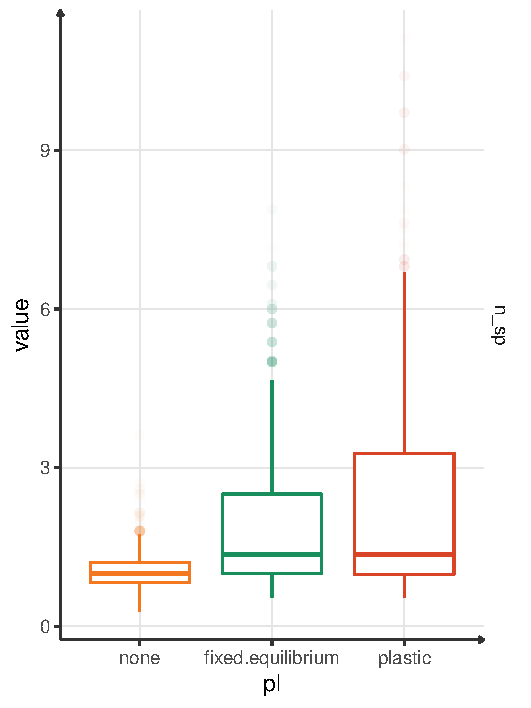
\includegraphics[]{./2_PP/Figures/Comm/comm_n_sp_differences.pdf}
\caption[Relative species richness in plasticity treatments]{Relative species richness in the three plasticity treatment. To negate the variability due to the parameter sets, the realised number of species is divided by the median number of species in \textit{non plastic} treatment for each parameter set. The variability is due to random invasion and climatic variability (inter-sites and inter-seasons).}
\end{marginfigure}

The effect of plasticity on coexistence is driven by the benefits of plasticity at the individual scale. These benefits are mitigated by the cost of plasticity, particularly the maintenance cost that affect all species relatively to their potential plasticity (proportional to $ 1- \tau$).

%Plasticity is responsible for high portion of variability, but also parameters: plasticity cost parameters:


Low values of plasticity maintenance cost (see figure \ref{fig:pl_cost}) show higher diversity for both plastic allocation algorithms. This trend is consistent across sites despites some inter-annual variability in the diversity. The effect is a bit less stronger for \textit{fixed-equilibrium} than for \textit{plastic-optimisation} (as already observed in figure \ref{fig:species_richness}). It is also important to notice that the cost of the plasticity has no negative impact on the coexistence levels for \textit{non plastic} simulations.

\begin{figure}%[tb]
%    \classiccaptionstyle
%\sidebysidecaption{0.60\textwidth}{0.3\textwidth}{%
    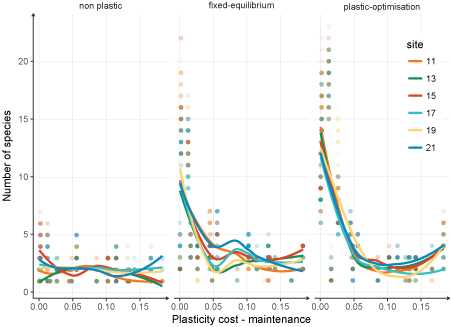
\includegraphics[width=1\linewidth]{./2_PP/Figures/Comm/comm_n_sp_pc_m_edit.png}%
%}{%
  \caption[Maintenance plasticity cost effect on species richness]{Effect of the cost of plasticity-maintenance on the absolute number of species in the three plasticity treatments. Individual season values (points) and site-specific trends (gam smoothing line) are represented. }
  \label{fig:pl_cost}
%  }
\end{figure}

%Consistent trends between sites. Inter-season variability (why didn't I save the weather?). Not super clean. Similar (but lower start) for plastic distance diversity. Can be because of interactions %or because non variable enough.

%Why higher diversity: it is not because of higher density (number of individual per m2).
%But changes in filtering: more species

The mechanisms through which the phenotypic plasticity impacts species richness are multiple (see figure \ref{fig:plasticity-effect} in chapter \ref{part:literature}). However it is hard to disentangle them all.


%\begin{figure}\label{fig:tiller_density}
%    \classiccaptionstyle
%\sidebysidecaption{0.3\textwidth}{0.6\textwidth}{%
%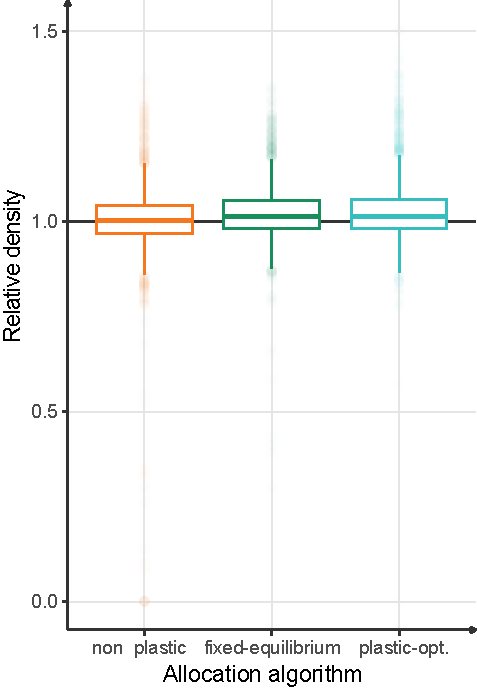
\includegraphics[]{./2_PP/Figures/Comm/comm_n_indiv_differences.pdf}
%}{%
%\caption[Relative plant density in plasticity treatments]{Relative plant density in the three plasticity treatment. To negate the variability due to the parameter sets, the realised number of plant is divided by the mean number of plant in \textit{non plastic} treatment for each parameter set. The plant density is estimated with the output of the reproduction process.}
% }
%\end{figure}

%The increase in plant density could impact the species diversity by an increase sampling \cite{lepik_high_2005}, or a increase competition intensity.

\begin{figure}%[tb]
%    \classiccaptionstyle
%\sidebysidecaption{0.5\textwidth}{0.4\textwidth}{%
    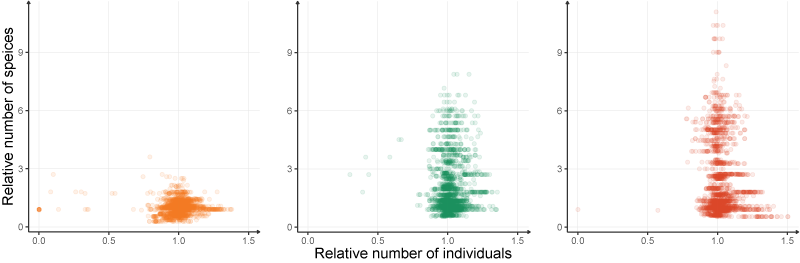
\includegraphics[width=1\linewidth]{./2_PP/Figures/Comm/comm_n_sp_n_indiv3.png}%
%}{%
  \caption[The species richness relative to the plant density]{The species richness against the plant density for the three plasticity treatments. To negate the variability due to the parameter sets, the variables are divided by the mean value for the \textit{non plastic} treatment for each parameter set.}
  \label{fig:species_per_plant}
%  }
\end{figure}

The plant density can be affected by the phenotypic plasticity leading to higher species diversity\parencite{lepik_high_2005}, leading to the sampling of more numerous species. The density, estimated by the number of individual after the reproduction phase (persisting individuals and produced seeds), is consistently higher in \textit{plastic} simulations (data not shown, but see figure \ref{fig:species_per_plant}). But the difference is relatively low (around 3\% higher than the \textit{non plastic} median density) and an order of magnitude lower than inter-annual and inter-site variations that can go up to 40\% difference relative to the median density (for any given parameter set). Moreover, the species richness shows no evident relationship with the density of plants in any of the algorithms (see figure \ref{fig:species_per_plant}). In addition, the number of individuals is greatly depending on the seed input parameter (strong linear correlation), but this parameter has no consistent effect on the species richness (data not shown).


%\paragraph{Plasticity selection}

%Not done yet. when is plasticity selected: is there a correlation between environment variables (or variations and plasticity selection). trade-off with other traits ?
\paragraph{Productivity}

The productivity may also be impacted by the phenotypic plasticity at the community level. Multiple mechanisms can be involved, but in any case a higher productivity is achieved by a higher efficiency in the use of the resources given. The plasticity can affect this efficiency at the individual level (with positive effects as observed in section \ref{chapter:individual}) or at the community scale with changes in the dominant species, plant density and competition intensity.

\begin{marginfigure}\label{fig:total_BM_comm}
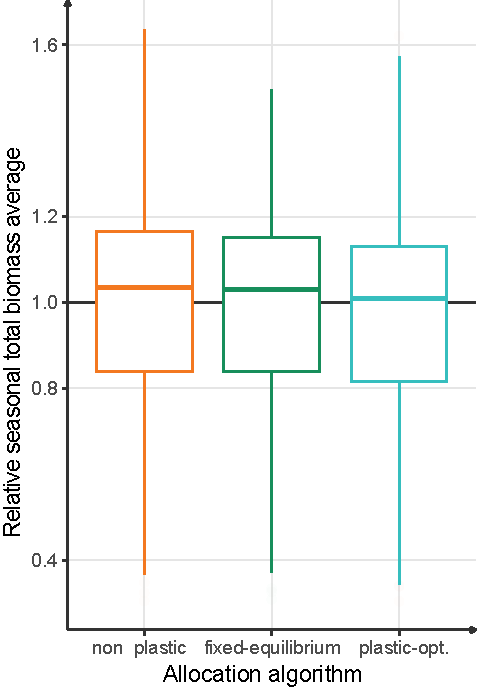
\includegraphics[width = \textwidth]{./2_PP/Figures/Comm/comm_BMtot_differences.pdf}
\caption[Average total biomass in plasticity treatments]{Average total biomass relative to  \textit{non plastic} simulations, in the three plasticity treatments.  To negate the variability due to the parameter sets, the variable is divided by the mean value for the\textit{non plastic} treatment for each parameter set.}
\end{marginfigure}

The productivity of the \textit{non plastic}, \textit{fixed-equilibrium} and \textit{plastic-optimisation} allocation algorithm show little differences. The \textit{non plastic} simulations average biomass tend to be a bit higher in certain cases. Like the diversity and density, the normalised yearly average are used to do the comparison, but the average biomass does not show great variations between plasticity, with a higher variability between sites and seasons. \textit{Non plastic} and \textit{fixed-equilibrium} median are quite similar, and the \textit{plastic-optimisation} show lower productivity than the other two algorithms. Both the conserved average plant biomass and the constant plant density lead to a constant community net productivity.

%\paragraph{Community structure}
%
%Because changes in community structure, no changes in density or productivity but, changes in structure, and competition evenness.
%
%\begin{figure}%[tb]
%%    \classiccaptionstyle
%%\sidebysidecaption{0.60\textwidth}{0.3\textwidth}{%
%    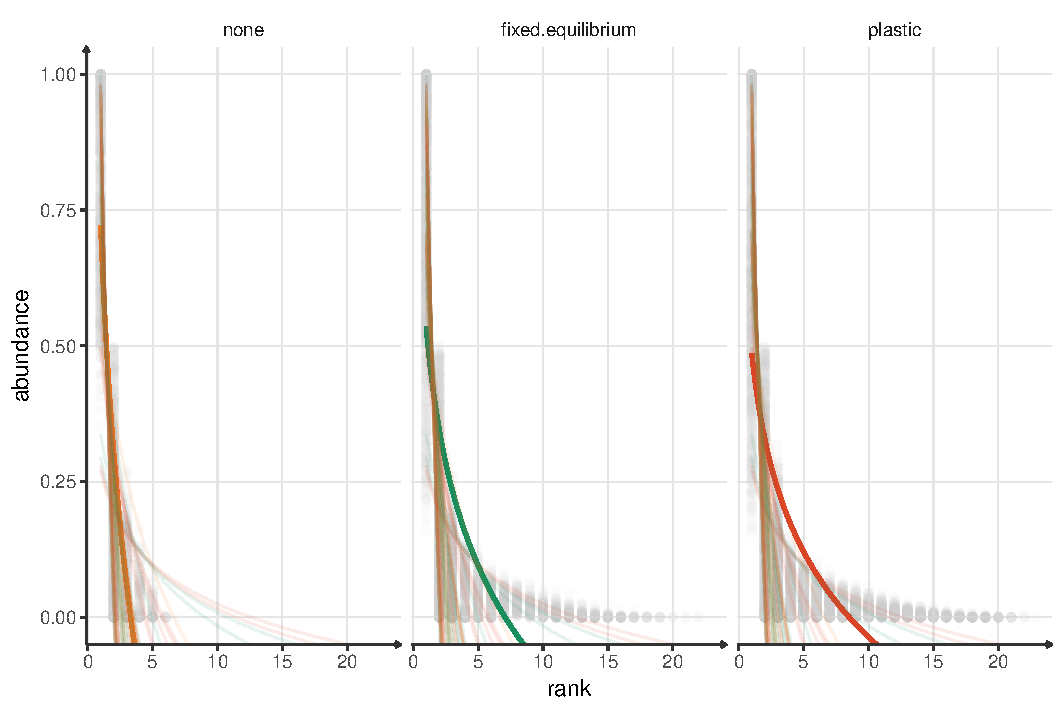
\includegraphics[width=1\linewidth]{./2_PP/Figures/Comm/comm_RAC_pl.pdf}%
%%}{%
%  \caption[Rank-Abundance curves fits]{Rank-Abundance curves.}
%  \label{fg:RAC}
%  %}
%\end{figure}



\paragraph{Plasticity: a winning strategy ?}

\begin{marginfigure}\label{fig:tau}
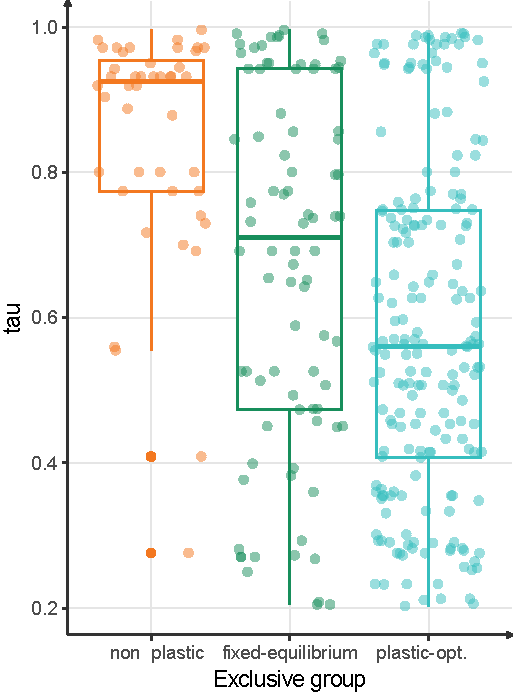
\includegraphics[]{./2_PP/Figures/Comm/comm_tau_differences_exclusive_groups.pdf}
\caption[Plasticity levels in exclusive groups]{Plasticity levels of species that are present in only one type of plastic treatment. Each point represent one distinct species.}
\end{marginfigure}

The allocation algorithm is expected to alter the fitness of potentially plastic plants. The selective effect of the allocation algorithms is investigated by plotting the $\tau$ value of species that are maintained in only one of the algorithms (in figure \ref{fig:tau}). Because of the plasticity cost, the selection of species with low values of $\tau$ signifies an improvement of the fitness due to plasticity. The distribution of $\tau$ is fairly high for \textit{non plastic} species and almost 75\% of the species have a value above 0.8, whereas \textit{fixed-equilibrium} specific species have lower values ranging from 0.2 to 1 with the median arond 0.7 and the \textit{plastic-optimisation} species have even lower values with a median around 0.55.
%Are plastic species more selected than the other ? Probably a bell-shape curves



There is a selective effect of the allocation algorithm on the axis related to the plastic strategy, but the resource-use strategies could also be impacted.

%\section{Strategy}

%\subsection{Results}
\paragraph{Variable strategies}

After the productivity and the diversity, the identity of the communities is investigated.

The mean and median values of the CWM of the resource-use strategies (PAR and PAS) do not show any shift between non plastic and fixed-equilibrium algorithms (table \ref{table:comm_strat}). The strategy variability is lower for the root strategy, than for the shoot strategy. The variability is relatively high compared to the differences between the two algorithms. The plastic algorithm show low values for the mean and median, with high variability.

Root strategies show high values (around 0.8) of active tissue allocation is all algorithms, in contrast with lower values of the shoot allocation of active tissues (around 0.6).

\begin{table}[]
\centering
\caption[Tissue resource-use strategy at the community level]{Summary statistics (mean, median and standard deviation (SD)) of the community weighted-mean of resource-use strategies in root (PAR) and shoot (PAS) for the three main allocation algorithms.}
\label{table:comm_strat}
\begin{tabular}{l|ccc|ccc}
                      & \multicolumn{3}{c}{PAR} & \multicolumn{3}{c}{PAS} \\
Variable              & Mean  & Median & SD     & Mean   & Median  & SD    \\ \hline
Non plastic           & 0.801 & 0.823  & 0.0733 & 0.644  & 0.657   & 0.152 \\
Fixed-equilibrium     & 0.804 & 0.823  & 0.0714 & 0.653  & 0.657   & 0.143 \\
Plastic\_optimisation & 0.749 & 0.778  & 0.133  & 0.589  & 0.600   & 0.200
\end{tabular}
\end{table}


Unlike the diversity, the identity of the community, defined by the dominating species, does not show a clear shift under plastic allocation. The great variability observed for each algorithm can be easily decomposed and explained because it is linked to the community structure and the dominant species. To decompose this variability in the identity, the community weighted mean 
%Select different strat? meh, from very site specific strats (one dominant species), to more variable within the site, but less differences between the strats. Shift from beta diversity to alpha diversity.
To analyse this variability, the community weighted means (CWMs) for the proportion of active tissues in roots (PAR) is visualised along time for the 6 sites, for 5 representative parameter sets (see figure \ref{fig:comm_strat}). The variability is decomposed between the spatial and the seasonal variability. Under \textit{non plastic} allocation, the CWM values for PAR are stable during time, but contrasted between sites. In contrast, under \textit{fixed-equilibrium} and \textit{plastic-optimisation} allocation, the temporal variability is greater, but the site specific means are closer. This pattern is reproduced for the shoot resource-use strategy (data not shown).


The differences in community structure certainly explain these contrasted source of variability of the community identity. The structure is altered by the increased species richness under plastic allocation (see figure \ref{fg:comm_str}), leading to a reduction of the abundance of the most dominant species, in addition of a long tail of the rank-abundance curves due to numerous species with low abundances.

\begin{figure}%[tb]
    \classiccaptionstyle
\sidebysidecaption{0.5\textwidth}{0.4\textwidth}{%
    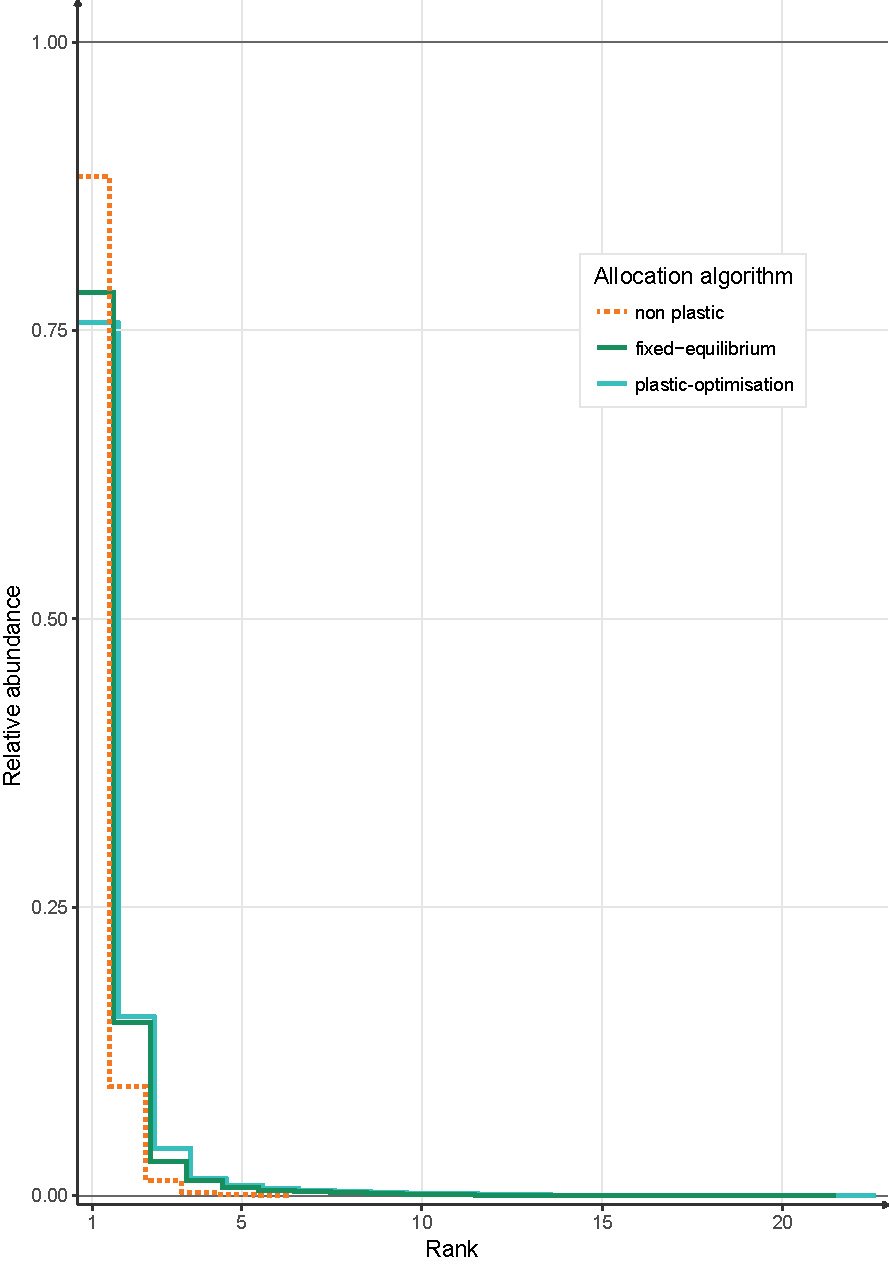
\includegraphics[width=1\linewidth]{./2_PP/Figures/Comm/mean_com_str2.pdf}%
}{
  \caption[Rank abundance curves for the three allocation algorithms]{Rank abundance curves for the \textit{non plastic} (\textcolor{myOrange}{- -}), \textit{fixed-equilibrium}  (\textcolor{myGreen}{--}) and \textit{plastic-optimisation} (\textcolor{myBlue}{--})algorithms. They illustrate the structure of the communities highly dominated by one species in \textit{non plastic} simulations, and highlight the long tail of rare species in plastic communities.
  }
  \label{fg:comm_str}
  }
\end{figure}

This shift in structure at the community scale, but also at the meta-community scale suggest a strong effect of the allocation on the overall structure of the ecosystem.
%Lead to changes in strats? If yes, is it direction\\
%al, or is the direction depends on species?%
%Do species change a lot there strategies?

%Is it always in the same direction for all species ? (reproduce Kichenin).


\begin{figure}%[tb]
%    \classiccaptionstyle
%\sidebysidecaption{0.5\textwidth}{0.4\textwidth}{%
    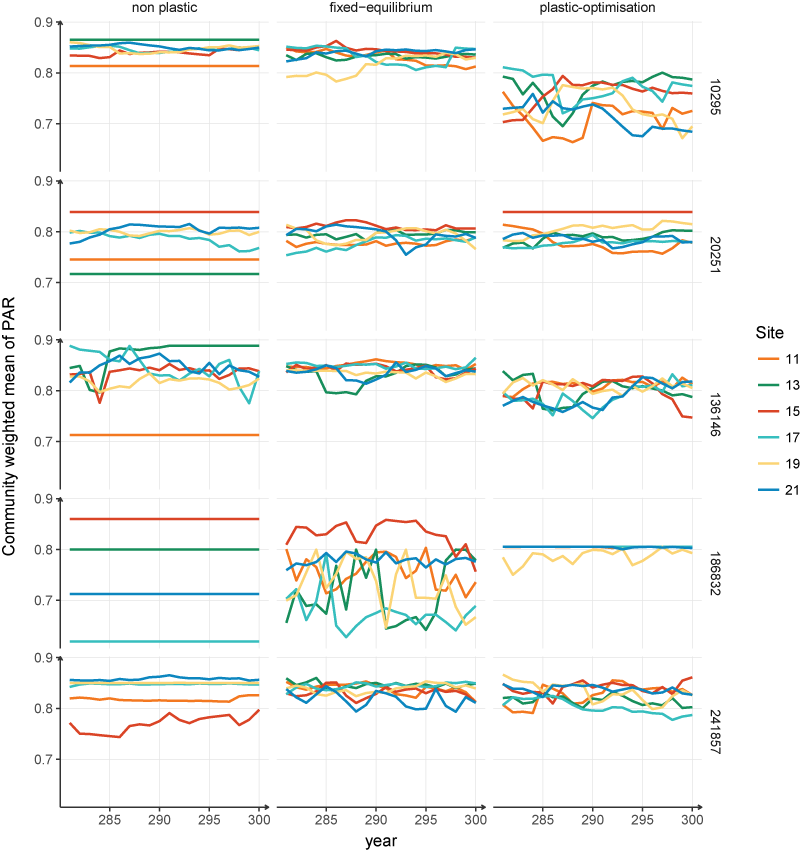
\includegraphics[width=1\linewidth]{./2_PP/Figures/Comm/comm_variability_lines.png}%
%}{%
  \caption[Spatial and temporal variability of the CWMs of the PAR]{Community weighted means of the proportion of active tissues in roots for each site, as a function of time and the allocation algorithm, for 5 representative parameter sets.}
  \label{fig:comm_strat}
%  }
\end{figure}


\paragraph{Different diversities}

% shift from beta to alpha diversity
Introducing plasticity in allocation leads to a shift in the diversity types. \textit{Non plastic} simulation tend to have more differentiated sites, captured by the high values of \textit{beta} diversity, but with low \textit{alpha} diversity as previously discussed (see figure \ref{fig:diversities}). 

\begin{figure}\label{fig:diversities}
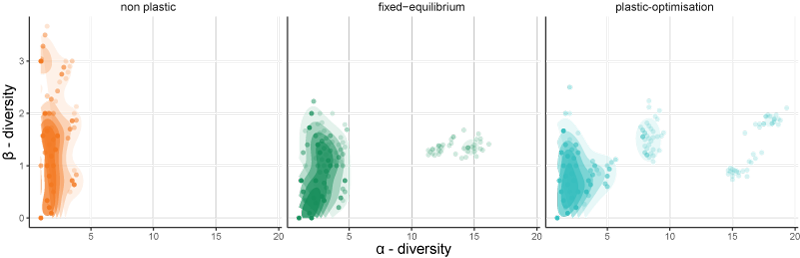
\includegraphics[]{./2_PP/Figures/Comm/comm_div_differences_alpha_beta.png}
\caption[\textit{Alpha} and \textit{beta} diversities as function of the allocation mechanism.]{\textit{Alpha} and \textit{beta} diversities as function of the allocation mechanism.}
\end{figure}

The total amount of species present over all sites and all seasons also varies between allocation algorithms, with a average total amount of 4.26 (median 4) for \textit{non plastic} allocation, of 7.69 (median 5) for \textit{fixed-equilibrium} allocation, and of 10.1 (median 4) for \textit{plastic-optimisation} allocation.


% what about functional diversity?

\subsection{Discussion}

%\paragraph{Competition evenness}

%The plasticity allows the emergence of new phenotypes that are plastic. Leading to higher density in competitors, and greater evenness. Hard to detect because not the same number of species, or require other experiments. 

\paragraph{Filtering} 
The great increase in the species richness observed under plastic allocation, for both the \textit{fixed-equilibrium} and \textit{plastic-optimisation} algorithms,  
results from a reduction of the strength of the filters. The results at the individual level analysed in the previous part suggest a weakening of the abiotic filter (1) as the importance of the plastic dimensions is reduced (static gain) and (2) variability in conditions can be overcome reducing the phenotype sensitivity to changes in resource balance (dynamic gain). In the other hand, the reduction of the abiotic filtering was anticipated to increase the competition intensity as more plants can settle in a given habitat. The reduction of the fitness differences observed at the individual level may explain a reduction of the competition exclusion despite a increase in the competition intensity. However it is relatively difficult to quantify the relative importance of competition relative to the abiotic filtering as they both are they both alter the resource levels. The overall reduction of filtering suggest a greater importance of the abiotic filtering reduction compared to the increase in the competition exclusion.

%Specific simulation experiment designs varying the dispersion of the strategies of the invading species could help disentangle these effects.  Detail these experiment and results interpretations

The absence of changes in the plant density, together with the stability of the community productivity, support the idea that if the abiotic filtering is reduced, it goes with an increase in the competition intensity. Therefore, the increase in species diversity is explained by a shift from a non uniform abiotic filter, to a more uniform biotic filter. Better understanding of the interactions between species strategies, and how they are modulated by plasticity could help building such interpretations at a higher level based on existing theories \parencite{chesson_mechanisms_2000}. 
With this perspective from the coexistence theory, we could explain the high diversity by the effect of the plasticity as an equalizing mechanism. Phenotypic plasticity, by allowing species to converge toward better phenotypes or to resist stresses, maintain a certain fitness evenness between species favourising the coexistence. Also, while these species are maintained, stabilizing mechanisms such as intra-specific competition can play a bigger role. However, while the intra-specific competition is recognised as often more important than the inter-specific competition \parencite{macarthur_limiting_1967}, the resource-use strategies as they are implemented in \model have certainly hierarchical effects \parencite{kunstler_plant_2016} as some strategies are dominant in certain conditions. Establishing how the intra- and inter-specific competition balanced, \textit{i.e.} if limiting similarity or competitive dominance prevail is crucial to better understand the community assembly in this context. This aspect is also critical because plasticity can affect this balance as observed by \citet{bennett_reciprocal_2016}. The current implementation of \model offers specific functions dedicated to paired simulations to evaluated the competitive and facilitation interactions. This tool can also be used to determine the transitivity properties of these interaction that can affect the ability of the model to maintain stable coexistence \parencite{levine_beyond_2017}. 


Finally, the fact that the species richness is not altered by the cost of the plasticity for \textit{non plastic} simulations (making certain phenotypes non viable), but is altered under plastic allocation, supports the fact that the species richness effect results from the allocation algorithm rather than the plasticity cost.


\paragraph{Productivity \& density}

% same level of prod, low increase in pl: probably sub-opitmum convergence
As mentioned, the productivity is mostly conserved between the allocation algorithms, as well as the plant density. I hypothesise that the increase in competition compensates the static and dynamic gains provided by the plasticity. It suggests that under \textit{non plastic} allocation, the carrying capacity of the sites is reached and that it cannot be exceeded despite the potential increased efficiency provided by the phenotypic plasticity. Because there is no change in the mean density, the mean resourcec-use efficiency at the scale of the plant should be similar. As analysed in the previous section, the plant efficiency can be limited by: the individual organ-specific efficiencies, the unbalance between organ activities or the resource use general level.  Disentangling the component of efficiency should allow to better understand the limits of the productivity. The plasticity may have a greater effect on the plot productivity under specific circonstances of strong disturbances, thanks to a higher resilience to drought or grazing events \parencite{maire_plasticity_2013}. On the other hand, it could be that the increase in competition leads to a decrease in resource-use efficiency as explained by the game theory \parencite{farrior_competitive_2014}. But the absence of clear differences in resource-use strategy does not support this hypothesis.

The density of plant is also unchanged. This is consistent with the stability in productivity. This stability in the plant density eliminates any sampling effect that could explain an increase in the observed species number for a given plot area as observed in \citet{lepik_high_2005}.

\paragraph{Does identity matter?}

Individual level results suggest the importance of the resource-use strategy for the success of the growth in different conditions. This idea seems to be validated by the observation that different species dominate different sites under \textit{non plastic} allocation. However, this pattern disappear under any of the two plastic algorithm tested. Thus, the root-shoot balance is probably more important in the selection of the success of the species.

Considering the variability of the weather during the season, the asymmetric dynamic gain should have promoted more exploitative species under plastic allocation. However, no convincing differences can be detected between the average CWM resource-use strategies between \textit{non plastic} and \textit{fixed-equilibrium} algorithms, for shoots or roots. This surprising result suggests that the differences in dynamic gain between strategies are not large between the different strategies. This result could also be explained by the stronger effect of the RMF axis (compared to the PAR and PAS) that lead to a low sampling of the other axis and hide potential effects of small amplitude. This effect can be exacerbated by the strength of the trade-offs (already noted in the previous chapter) that limits the number, and thus diversity, of viable strategies. This problem also limits our ability to interpret the differences between shoot and root successful allocation strategies to active tissues, because they may results from strong parameter effects rather than a difference in the sensitivity of the two organs. Similar experiences as in the previous chapter (analysis of the best strategies along a gradient), but including shoot strategies may enable us to compare the relative importance of the two activities in the context of community simulations.

The \textit{plastic-optimisation} algorithm shows lower values for shoot and roots proportions in active tissues. However, because the values use to compute the CWMs do not take into account the plasticity in these traits (for technical reasons, the expressed trait values are not recorded), this difference is artificial and does not reflect changes in the dominant strategies.

The detection of the plasticity effect on the community identity can also be masked by changes in the structure of the communities.

% The absence of clear changes in the CWM identity (resource-use strategy) confirms 


\paragraph{Community structure}

The increase in the species richness necessarily comes with a change in the community structure under plastic allocation. This shift consist in the reduction of the dominance of the most abundant species, an increase in the second and third dominant species, as well as a longer "tail" with many species of low abundance. While the presence of numerous low abundance species could suggest marginal effects  of the plasticity allowing the maintenance of rare species at the border of their niche, the reduction of the relative abundance differences between the species dominating the community demonstrates a stronger effect. 
%Shift in community structure

This strong effect of the plasticity on the community structure explains the differences in identity variability under the two types of allocation algorithms. On one hand, under the \textit{non plastic} allocation, the identity varies mostly between sites, but stays fairly stable between seasons. On the other hand, the variability is temporal rather than spatial under \textit{fixed-equilibrium} or \textit{plastic-optimisation} allocation. Because the niches are narrow without plasticity, the small climatic differences between the sites lead to different compositions and high spatial heterogeneity in the community identity. The strong filtering force that constitute the changes in conditions does not allow species at low density to establish. The extinction of these species releases the competition intensity after a climatic stress event, offering more resources for the dominating species that translates into a large reproduction effort. Because of storage effect, and strong abiotic filtering, the dominant species is favoured even in bad years. The combination of the sensitivity of the fixed phenotypes to changes in conditions with population dynamics favours stable low diversity communities. Under plastic allocation, the niches are wider, allowing more species to invade and survive a given habitat, despite changes in conditions. Because they have wider niches, and the climatic conditions between sites are not that different, the chance that they invade multiple sites are higher than in \textit{non plastic} allocation. Because more species are present, and the competition is more even, the seasonal variations in conditions allow changes in the relative abundance of the species while the community composition is stable. These changes alter the community weighted means and therefore the identity of the community. The differences in species composition and the effects on the CWM of PAR for the three allocation algorithms are illustrated in the figure \ref{fig:explain_strat}.

\begin{figure*}\label{fig:explain_strat}
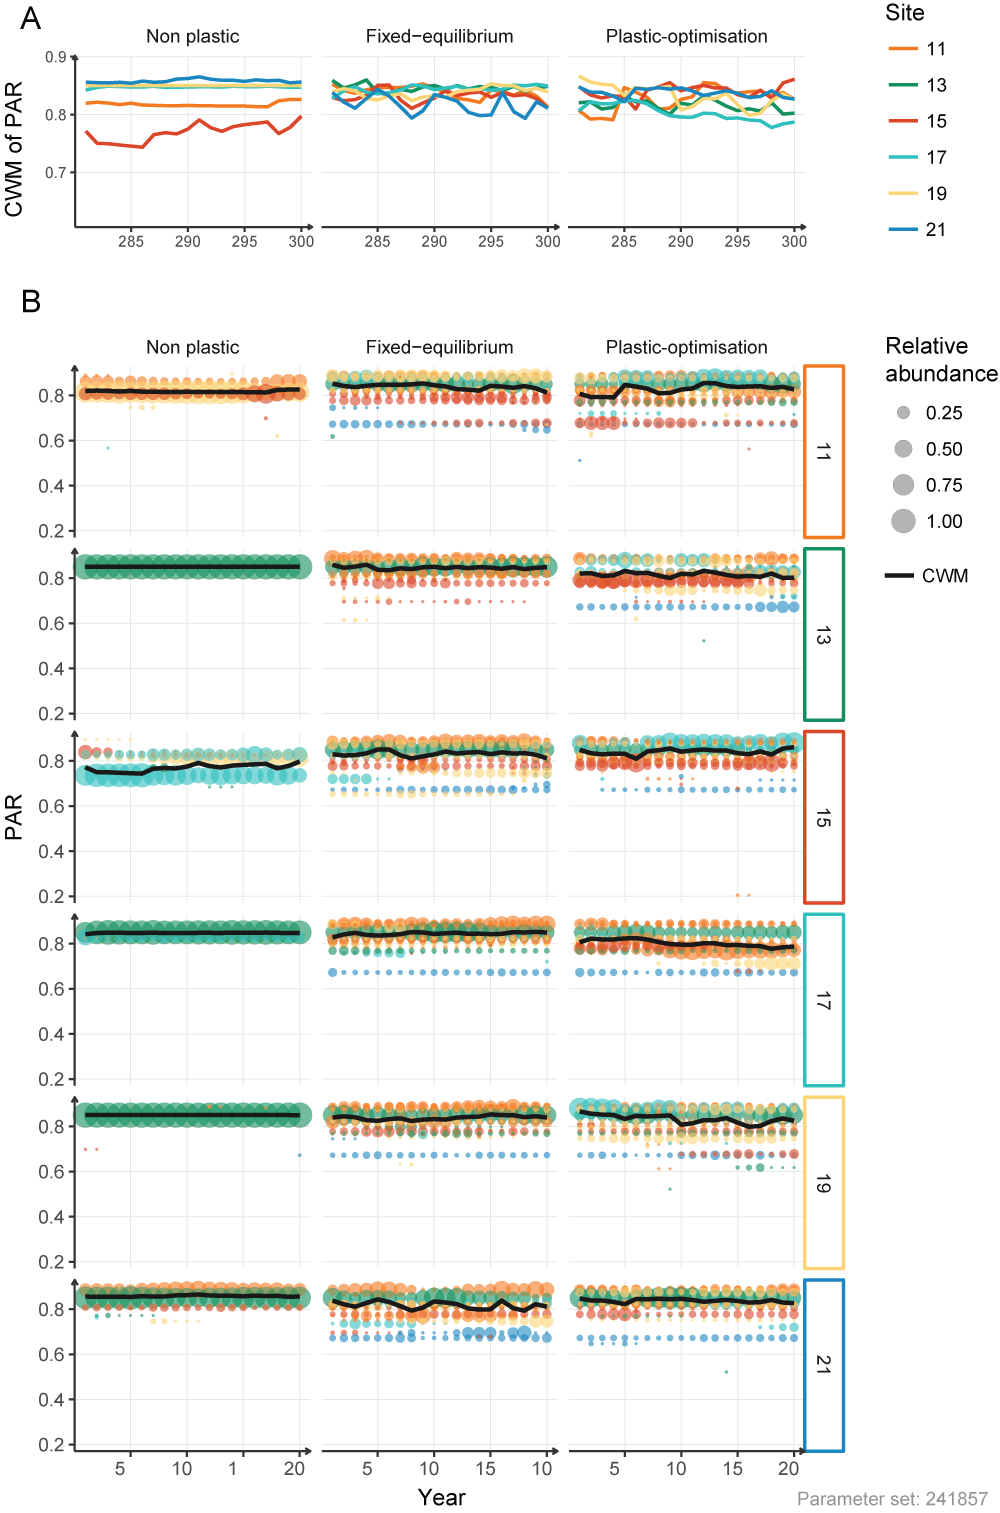
\includegraphics[]{./2_PP/Figures/Comm/explain_par_variability.png}
\caption[Effect of the community structure on the inter-site variability of the community identity.]{Inter-site and inter-season variability of the community identity (A) explained by the effect of the plasticity on the community structure (B).}
\end{figure*}
 

%The allocation algorithm, by impacting the niches and the importance of the abiotic filtering, controls the mechanism driving the community structure.

%also, Jung \cite{jung_intraspecific_2014} show contrasting response between species and within species - might not be the best 

\paragraph{Different forms of diversities}

The structural changes in the community and meta-community can be seen with the perspective of the diversity. While many diversity indexes could be used to decompose and analyse the diversity of such communities, these simple indexes (\textit{alpha} and \textit{beta} diversity indexes) are sufficient for this level of analysis and to express the differences in the structure of the ecosystem caused by the allocation algorithms.

%why higher alpha div
The increase in \textit{alpha} diversity has already been discussed and results from a niche widening (or a reduction of the abiotic filtering). The beneficial value of the plasticity to explain this increase in \textit{alpha} diversity is demonstrated by the significantly lower value of $\tau$ for the species unique to one of the two plastic algorithms for each parameter set. 
% Talk about species TO and tau.


The lower total number of species over all sites demonstrates that the reduction of the \textit{beta} diversity is explained only by the differences in \textit{alpha} diversity. This interpretation is coherent with the conclusion that the niche overlapping induced by the phenotypic plasticity explains most of the community dynamics patterns.

%The implementation of more realistic meta-community dynamics, with explicit invasion from site-specific seed-rains, may alter these patterns. Under a close meta-community dynamics, the large overlapping between local communities may be reinforced under plastic allocation. Under non plastic allocation, such dynamics could (1) re...

%The decrease in beta diversity is explained by the larger overlap between community, caused by a larger overlap between species niches. Such effect could even be reinforced by a different implementation of the link with the meta-community. In this set of simulations, the meta-community is composed of the initial set of species, evenly abundant, where invading seeds are randomly sampled. A different approach could be to consider all sites connected, and sample the invading species from the seeds produced in the other sites. In the case of the \textit{non plastic } allocation, because the sites are highly dominated by one species and the site specific conditions generally do not match the narrow niches of the species, a low number of non adapted seeds would not be able to invade the other sites, and reduce the possibility of coexistence relative to a sampling from a much richer meta-community. This would accentuate the contrast between the alpha and the beta diversity. Under plastic allocation, the community share multiple species, if the seed dispersion is limited to the seed produced within the sites, there would be a large redundancy and a low turn-over in the incoming species (relative to a random sampling from a large meta-community) leading to a very low beta diversity. By affecting the niches and therefore the relative distance between sites in the "niche space", the phenotypic plasticity greatly alters the structure, not only of the communities, but also the meta-community.

%Plasticity allows for bigger niche (variability dimension), more chance to build enough "growth potential" to persist. Otherwise, other species that are dominant, because other species can settle, take advantage of it.
%Should look at the growth rates hierarchy for a couple of simulations.

% but also lower beta


% diversity indexes

% What does it mean to modelling and to community properties ?



\paragraph{Statistics}

The allocation algorithm is only one of factors that impact the response variables that are analysed in the previous sections. The parameter sets and climatic variables (year and sites for community-level simulations) also greatly impact the outcome of the simulation. While the perfect knowledge of the model and the total control over the simulations allow us to decompose and disentangle all these effect, the focus has been on the effects of the allocation algorithm, relative to the other effects. As mentioned in the method, the normalisation relative to the mean of each parameter set eliminates partially the complex effect of the numerous parameters on the scale of the variables, while keeping the overall behaviour (reduction, increase or stability). It also allow to compare the effect of the algorithm relative to the other factors source of variations (season and site). Maybe another normalisation could have been performed (standardisation), but this methods seems to provide already consistent information.

Ones could regret the lack of statistical analysis to estimate the significance of the effects. But, as mentioned the total control and knowledge of the model would allow to ensure significance results for any test, and therefore is not informative (see \citet{white_ecologists_2014} for extended arguments). While the effect size could have been calculated, the graphical representations produced provide enough information to estimate these effect size and compare the effect of the explicative variable of interest (allocation algorithm) to the variability caused by the other factors. 

I believe the representation of the model outputs through specific visualisations gives a better understanding of the general behaviour of the model, as well as an intuition of the unique differences between the different conditions, than large tables and statistical test could do in this context. 
%Interaction between plasticity effects and parameter sets, but the interest here, even if  it is interesting. Higher variance due to site and weather. The almost perfect knowledge of models allows an extremely precise decomposition of the effects, but at the risks of loosing broad effects. The difficulty is to measure the relative strength of these effects, and generalise. But, by essence, the parameters are suspected to have a significant effect that can be identified, otherwise it would not have been included in the model.

% need to reread that, but decomposed when possible, needed, or to show consistency. Not always, to make the description and message clearer.  white_ecologists_2014 : no statistical tests



\paragraph{Plasticity \& community properties}

\textbf{The introduction of phenotypic plasticity has many effect of community-level process, with consequences on the main properties of the communities (see figure \ref{fg:comm_pl_effect}). It reduces the filtering role of abiotic conditions, increasing the competition intensity, but it also decrease the fitness differences (or increase the competition fairness) leading to higher \textemph{species diversity}. The overall plot productivity does not seem to be affected by the allocation algorithm, This is explained by multiple factors: the absence of differences in plant density, similar resource-use strategies that maintain the overall tissue-efficiency, and the increase in competition intensity that compensates for potential increase in efficiency due to balanced activities. The identity was not impacted by the allocation algorithm, unlike the structure of the communities and meta-community, leading to a shift from \textit{beta} to \textit{alpha} diversity, and from inter-site to inter-season variability of the resource-use strategy.}


\begin{figure}%[tb]
    \classiccaptionstyle
\sidebysidecaption{0.5\textwidth}{0.4\textwidth}{%
    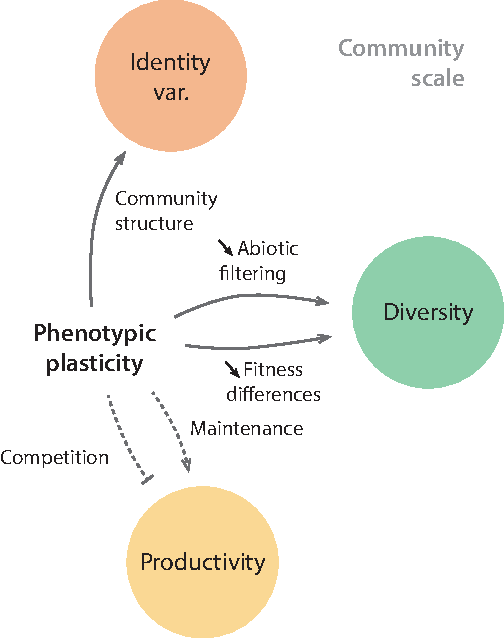
\includegraphics[width=1\linewidth]{./2_PP/Figures/Comm/comm_pl_effect.pdf}%
}{%
  \caption[Effects of the phenotypic plasticity on the community properties]{Effects of the phenotypic plasticity on the main properties of the community.}
  \label{fg:comm_pl_effect}
  }
\end{figure}


\paragraph{Robustness}

The simulation at the scale of the community produce surprising results. Imagining how stable these patterns would be under alternative implementations can give us an idea on how robust these results are. The two alternative implementations suggested are presented in the previous chapter. 

On one side, the structure and diversity differences are explained by two main mechanisms: the reduction of the abiotic filtering and the reduction of fitness differences. The equilibrium architectural plasticity (I1) has the ability to maintain organ activity balance, while increasing the performance of foraging strategies. This efficiency \parencite{maire_plasticity_2013} guarantees the reduction of the abiotic filtering. The stres-based plasticity with reaction norws should also be able to reduce the abiotic filtering under the condition of the selection of sensible reaction norms. These reaction norms even have the potential to better stabilise the plant efficiency by regulated the overall plant acitivty, and not just the balance between the activity of the organs. ON the other hand, the diveristy is also promoted by the reduction of the fitness differences. The reduction of the sensitivity to changes in conditions partly explain this effect, but the convergence of the phenotypes also explains this reduction. While both alternative implementations should reduce this differences in fitness by reducing the sensitivity of the phenotypes to changes in conditions, the reaction norm implementation (I2) should limit the phenotypic convergence by the diversity of the reaction norms in presence. The contrasted strategies of avoidance versus tolerance should participate in the maintain of functional diversity. This reduction of the convergence may limit the reduction of fitness differences promoting the coexistence \parencite{chesson_general_2000}. On the other hand, phenotypic plasticity may enables niche partitioning as observed in empirical data \parencite{zuppinger-dingley_selection_2014, roscher_contrasting_2015}. The beneficial effect of the phenotypic plasticity, because it is constrained by trade-offs allowing coeistence \parencite{tilman_niche_2004}, should favour coexistence in most conditions.


Both algorithms have potential for greater efficiency. This efficiency may affect the productivity in a larger way than the current implementation \parencite{maire_plasticity_2013}. A finer exploration of the response of the community after disturbance events should give us better understanding of the effect of the plasticity on productivity stability \parencite{richter_phenotypic_2012} on grassland systems.

Because the \textit{alpha} diversity is expected to be impacted in a similar way than in the current state of the model, structural changes of the communities and meta-community are susceptible to be reproduced in the different implementations. The identity of the community, expressed as the CWMs for the resource-use strategies may however be impacted. Indeed, the impact of competitive species under architectural plasticity may be stronger, with either a rapid competitive exclusion of the subordinate species, or the rapid shortage in resources leading to more conservative species dominance. The reaction norm plasticity, by allowing more diversity in the plastic response may also have a drastic effect on the community identity. The complexity of the interactions and resource dynamics introduced by these implementations does not allow the anticipation of the effects on the community identity. At the contrary, it further encourages us to try alternative implementation of plasticity to unravel all these processes.

%Is it robust ?

% niche differentiation
%Among the \cite{roscher_contrasting_2015} + jena and diversity (tilman)

\paragraph{Strategic plasticity}

The plasticity as a strategy defended in the chapter \ref{part:model}, that makes the plasticity an axis of strategic differentiation, is only superficially studied here. The figure \ref{fig:tau} shows the average phenotypic stability value for algorithmic specific species (only reproduce in one of the algorithms). This results confirms that plasticity favours species with lower tau values. The particular relationships that may exists between levels of plasticity, the two distinct costs and the temporal variability of conditions should be investigated to better understand the role of the plasticity costs as a limit of the phenotypic plasticity \parencite{dewitt_costs_1998, auld_re-evaluating_2009}.

The adaptative value of the different levels of plasticity can be measured by the distribution of the $\tau$ values against gradients of resource variability, allowing hypothesis testing on the limits of the plasticity.

\subsection{A broader perspective on phenotypic plasticity at the community level}

\paragraph{Services and global change}

The strength of models as tools is to help us understanding the underlying mechanisms, but also to project the system of interest in alternative scenarios. While this subject is further discussed in the next chapter (chapter \ref{part:synthesis}), the current results can still be analysis with this perspective.

The phenotypic plasticity effects at the community level mostly affect the community structure and diversity. The addition of multiple rare species, while they do not participate greatly to the productivity, they still provide numerous benefits. The species diversity can for example support a flower diversity that promote cultural services, as well as honey production. This flower diversity is also tightly linked to the pollinator diversity \parencite{frund_pollinator_2010} themselves enhancing the persistance of plant communities \parencite{fontaine_functional_2005}. Such positive feedback mechanisms have essential positive feedback effect stabilising the coexistence. 

The species diversity has multiple other benefits (see chapter \ref{part:literature})\parencite{tilman_diversity_2001}. One of these effect is to enhance the stability of the community \parencite{morin_temporal_2014}. This effect is even more important in the context of the climate change. The shift in climatic conditions driven by the climate change may put some species outside of their fundamental niche. Such effect can lead to critical transitions \parencite{scheffer_catastrophic_2001}, especially in case of low diversity and narrow niches, where the equilibrium state is fragile. In this context, the phenotypic plasticity have two beneficial effects: (1) it widens the fundamental niche of the species, reducing the risk for rapid shifts, (2) increases the species diveristy, allowing subordinate species to become dominant \parencite{adler_climate_2006} with potential effects on community's stability. Also, while no net effects could be detected on the average productivity, the size of the seed rain may be affected, weakening the stability of the system and increase its vulnerability to plant invasion.

The modification of the meta-community can also have an impact of the response to global change. The high redundancy in species between site, while it decrease the \textit{beta} diversity, also support the site stability. Indeed, in case of discriminated communities (communities are composed of unique and different species), any local transition leading to the local extinction of the species also leads to the extinction of the species at the meta-community level. Whereas, in redundant community structure, a local extinction can be reverse later thanks to invasion from undisturbed (or less disturbed) communities.

Redundancy and plasticity should also help smoother transition between states, and should allow management adjustment to be adopted. The potential effect on the resistance to alien species should also be investigated.


%2 perspective: differences between with and wtihout pl. Effect on plastic and on non plastic sp.
%
%% critical transition in non plastic communities
%\cite{scheffer_catastrophic_2001}
%
%% more stable because more diverse, closer communities
%\cite{morin_temporal_2014} \cite{tilman_diversity_2001}

% plasticity : more even competition : larger niche -> smoother transitions

% resistance to stress amplitude and frequency : more heterogeneous comm, either more resistant, or more plastic. until only resistance  less rapid shift in identity because asymmetric dynamic gain



% what about management : abandunment or fertilisation: 
% - abandonnement: less plastic species,  plasticity itself predict smoother transition
% - fertilisation : more exploitative, more plastic, could work better than expected if plasticity is considered.
%

\paragraph{The specificity of the mechanisms}

The development of this model also highlights the importance of the perspective on a phenomenon. One of the primary objectives of this work was to better understand the source and effects of intra-specific variability. This issue had received increasing importance \parencite{de_bello_quantifying_2011, albert_when_2011, violle_return_2012, siefert_global_2015}. And the question has been explored with empirical and statistical approaches \parencite{jung_intraspecific_2010,  jung_intraspecific_2014, bennett_reciprocal_2016}, and theoretical models that allow the examination of the underlying processes \parencite{hart_how_2016}.

Theoretical models are great tools that allow, by the simplification of the problem and the identification and characterisation of the processes, to explicit the mechanisms and quantify emerging properties of the system by the study of their mathematical properties. Such an approach was developed by \citet{hart_how_2016} to investigate the impact of the intra-specific variability upon the coexistence mechanisms. They show an overall negative effect resulting from numerous processes. A part of the explanation, the Jensen's inequality effect with species interaction coefficient, might be overcome by the fact that empirical estimation of these coefficient should capture this effect. But another argument resides in the modification of the relative strength between the intra-specific and inter-specific competition interactions. While the reasoning is valid, it relies on an assumption, the symetry of trait mediated competition. However, such assumption, deeply rooted in ecology \parencite{macarthur_limiting_1967} may not always be verified  \parencite{kunstler_plant_2016}. The other limitation of such approach is that it ignores the source of the variability. However, the validity assumption made on the higher level processes\sidenote{those that are impacted by the intra-specific variability, as opposed as those that cause this variability} may depends on the underlying mechanism. In \model the explicit description of the intra-specific variability as a result of the phenotypic plasticity allows to avoid assumption and test directly the effect of this specific form of intra-specific variability. It appears that the phenotypic plasticity does not limits the coexistence by reinforcing the inter- versus intra-specific competition, but rather diminishes the competitive differences between species \sidenote{among other positive effects}. This example highlight the strength of mechanisitic approaches to investigate complex processes of which the underlying drivers may be ignored at the level of observation. The work of \citet{zuppinger-dingley_selection_2014} is another example on the complex links between intra-specific variability\sidenote{here expressed by character displacement} and coexistence mechanisms. They highlight the effect of the diversity of neighbours on the trait expression of species, showing potential positive feedback loops between functional and species diversity.

Other forms of intra-specific variability must be investigated, but it is likely that genetic variability results from fine scale selection processes \parencite{hamann_evidence_2016}, challenging the hypothesis of theoretical models. The intrinsic limitation of these approaches resides in the assumption that the source of the intra-specific variability (\textit{e.g.} spatial or temporal heterogeneity leading to genetic variability or phenotypic plasticity) does not affect the common rule driving the interactions, while in many cases the interaction forces depend on the alteration of the conditions (see \citet{choler_facilitation_2001} along elevational gradient) that also explains the intra-specific variability (see \citet{kichenin_contrasting_2013} along similar gradient).

Mechanistic models should be used in complement of theoretical models. Theoretical models are easier to develop and test and may reveal interesting patterns. Mechanistic models can be used to investigated the underlying processes of those patterns. But these models rely on strong empirical knowledge, patterns and data, that are costly to gather. This knowledge and data also nourish the development of new theories and theoretical models. This interdependency illustrates the need for collaboration between the different approaches in order to build and test theories that mhelp us understanding the world around us.

%example with altitude gradient: kichenin and choler 2001
%\paragraph{Measures and rules}
%
%intra-specific variation : jensen inequality : with negative effects on coexistence. 
%
%Jensen's inequality: question of measure.
%
%pl =:source of variation: driven. There are causes to this variability. Supposing variability under constant rule does not make sense to me. Variability because non constant rules. Under non constant rules (climate, interaction coeeficients, stochasticity) pl has non linear effect (static gain benefit to non fitting species, or asymmetry in dynamic gain) but mostly favour the diversity.
%
%More genetic approaches for the genetic intra-specific var. effect (not just pl), but I on't think it is negative... at least more lickely to alter the source of vairability or the for mof diversity, as observed here from beta to alpha.
%
%measures and rules
%
%\paragraph{Intra-specific variability}
%
